\documentclass[sigplan,screen]{acmart}

%% \BibTeX command to typeset BibTeX logo in the docs
\AtBeginDocument{%
  \providecommand\BibTeX{{%
    Bib\TeX}}}

\setcopyright{acmlicensed}
\copyrightyear{2024}
\acmYear{2024}
\acmDOI{XXXXXXX.XXXXXXX}

%% These commands are for a PROCEEDINGS abstract or paper.
\acmConference[23rd ACM Workshop on Hot Topics in Networks (HotNets '24)]{}{Nov, 2024}{Irvine, CA}

\acmISBN{978-1-4503-XXXX-X/18/06}


\newcommand{\todo}[1]{\textcolor{red}{TODO: #1}\PackageWarning{TODO:}{#1!}}


\usepackage{graphicx}
\usepackage{subcaption}
\usepackage{float}

%%
%% end of the preamble, start of the body of the document source.
\begin{document}

\title{Q2: A Framework for Quantum Clouds}

\author{Shaun Ghosh}
\email{sounakghosh@umass.edu}
\affiliation{%
  \institution{University of Massachusetts Amherst}
  \postcode{01003-9284}
}

\author{Victor Lam}
\email{vslam@umass.edu}
\affiliation{%
  \institution{University of Massachusetts Amherst}
  \postcode{01003-9284}
}


\author{Ali Hamza Malik}
\email{ahmalik@umass.edu}
\affiliation{%
  \institution{University of Massachusetts Amherst}
  \postcode{01003-9284}
}

\renewcommand{\shortauthors}{Ghosh, Lam, Malik}


\begin{abstract}
\textbf{The rapid advancement of quantum and cloud computing technologiesop  presents a significant opportunity to revolutionize computing by developing a quantum cloud similar to the current cloud infrastructure. Development of a quantum network and cloud will see the emergence of a wide range of new technologies and (Quantum) Network Functions. This, however, can pose a big hindrance in the growth of quantum networks due to scalability and placement issues. To combat this we propose an application-agnostic scheduling framework, called Quantum Queue or Q2, for quantum packet processing in a quantum cloud by managing Virtualized Quantum Network Functions (QNFVs). By utilizing virtualization techniques, our solution guarantees efficient and flexible management of quantum network functions, facilitating seamless interoperability between existing quantum network functions and those yet to be developed. This framework lays the foundation for a scalable, heterogenous, and robust quantum cloud infrastructure, poised to support a wide range of applications and drive the future of cloud computing.
}
\end{abstract}

\keywords{Cloud Computing, Quantum Computing, NFV, SDN}

\maketitle

\section{Introduction}
The landscape of cloud computing has experienced tremendous growth and transformation over the past decade, becoming an integral part of modern technological infrastructure. With this growth, cloud providers such as Amazon AWS and Microsoft Azure have introduced services that offer access to quantum computing resources. As the capabilities of quantum computing expand, the concept of a dedicated quantum cloud—integrating quantum computing and quantum networks to form a cloud infrastructure similar to classical clouds—emerges as the next frontier in cloud technology.

Quantum computing, leveraging the principles of quantum mechanics, holds the promise of solving problems currently intractable for classical computers. This includes applications in cryptography, optimization, drug discovery, and complex simulations. To truly unlock the potential of quantum computing, it is imperative to develop a quantum cloud that offers native support for quantum operations, enabling more efficient and scalable utilization of quantum resources.

In parallel with these developments, the cloud computing paradigm itself has evolved, incorporating various network functions such as firewalls, load balancers, and traffic filters to manage and optimize data flow. These functions have become essential for maintaining performance, security, and reliability in cloud environments. Drawing on the principle of "ontogeny recapitulates phylogeny," it is expected that quantum clouds will similarly evolve to include their own suite of network functions tailored to the unique requirements of quantum computing. These Quantum Network Functions (QNFs) will be crucial for tasks such as quantum error correction, quantum key distribution, and the routing of quantum information.

Our project aims to address the emerging needs of quantum cloud computing by proposing an application-agnostic scheduling framework for quantum packet processing in a dedicated quantum network with virtualized Quantum Network Functions (QNFVs). This framework seeks to provide a comprehensive solution for the development of quantum cloud infrastructures, ensuring that quantum computing can be accessed and utilized as seamlessly as classical computing resources.

\section{Background}
\subsection{Quantum Computing}
Quantum computers differ from classical computers in that they use quantum bits (qubits) instead of classical bits. 
Qubits exist as either photons or electrons while classical bits are typically transistors. 
Transistors store information by being in either an on state (1) or an off state (0).
Qubits however are not limited to two states and can exist in a superposition of these states.
That is they can be in both the $\left| 0 \right>$ and $\left| 1 \right>$ state at the same time.
This is useful as their state can be modeled as a vector inside the Bloch sphere, which allows a qubit to store much more information.
The qubit's superposition however will collapse to one of the two states if it is measured.\\

The basis of quantum communication lies in entanglement.
We can entangle qubits such that the superposition of their states are "combined", meaning the measurement of one qubit gives us information about the other qubit.
For example, we can write their state as $\left| \Phi \right> = \frac{\left| 00 \right>}{\sqrt{2}} + \frac{\left| 11 \right>}{\sqrt{2}}$.
Here, the qubits are either both $\left| 0 \right>$ or they are both $\left| 1 \right>$.
If we measure the first qubit and find that it is a $\left| 1 \right>$, then the second qubit's state is known and it will collapse to this state.
With quantum communication, we need to entangle qubits and the qubits to both the receiver and sender.
Sending qubits is usually simply just sending a qubit encoded as a photon through a fiber cable.
However, fiber cables have attenuation and the "signal" weakens over time.
Due to the no-cloning theorem, we cannot make a copy of this qubit to amplify the signal.
We therefore need quantum repeaters, a device which performs entanglement swapping to break down long distances into a bunch of shorter segments instead.
Repeaters are the backbone of any quantum network, and it is analogous to a link in classical computing.


\subsection{Software Defined Networks}
Massive data centers and even networks of data centers can have millions of hosts and switches.
When each host has its own operating system and applications, the hosts and the network can become bloated.
Hosts each have millions of lines of code on a network with billions of gates.
Changes to the network hard to make and may take a while to fully propagate.
Software defined networks (SDN) \cite{sdn} provide a solution to this by taking the operating system and applications out of the host and making them global.
That is, the operating system has a global view of the entire network and controls the flow of packets by changing policies (e.g. forwarding tables) inside of network switches.
The primary benefit we are looking to draw from SDNs are the control plane advantages associated with having a global view of the network.


\subsection{Network Virtualization}
Network virtualization \cite{NV} is the movement of traditional network resources from hardware to software.
This includes NFVs and containerization of operating systems, allowing them to be dynamically deployed and scale as needed.
Like SDNs, network virtualization seeks to use hardware simply for packet forwarding with all other functions existing in software.
This differs from SDNs in that these resources still need to be managed; it is easier to manage when resources exist virtually as they can be deployed anywhere at anytime and are not bounded by the topology of the network.


\subsection{Elastic Edge}
% What E2 talks about
% What network functions we can implement
Elastic edge (E2) \cite{e2} is a framework enables application-agnostic packet processing.
Network function virtualization (NFV) allowed for easier scaling and management of network functions, but the management of many NFVs can be difficult.
E2 has three main components: the E2 manager, the server agent, and the E2 dataplane.
The manager oversees the entirety of the network while the server agent manages individual servers, and the E2 dataplane manages the processing of packets at each server.

This paper is the inspiration behind our work.
However, the ideas and techniques used in this paper are designed for classical networks and therefore require intricate thought when applied to a quantum network.


\subsection{Quantum Networks}
 Quantum networks \cite{Kimble_2008} leverage the principles of quantum mechanics to enable secure and efficient communication by transmitting quantum bits (qubits) over various media, such as optical fibers and free-space links. These networks utilize unique quantum properties like superposition and entanglement to perform tasks that are infeasible for classical networks, including Quantum Key Distribution (QKD) for unbreakable encryption and quantum teleportation for state transfer without physical transmission. The architecture typically involves quantum repeaters to extend communication range, quantum processors for handling quantum operations, and quantum memories for temporary storage of qubits. Quantum networks like classical networks have hosts (quantum computers, etc) and forwarding hardware (quantum repeaters, etc,). 

\subsection{Quantum Network Functions (QNF)}
Quantum computing being so different from classical computing requires its own set of network functions.
Qubits are especially susceptible to noise and entangled qubits can experience decoherence.
For any network to have reliable quantum communication, it would need to have quantum error correction.

Quantum entanglements can theoretically last forever, but they often suffer from decoherence due to their interactions with noise in the environment. 
As entanglements breakdown, we need to create new ones to be able to communicate.
Entanglement distribution is then a vital function in quantum cloud networks.

One function from classical clouds that are feasible to implement in quantum is load balancing. 
Load balancing is just as it sounds, distributing packets or qubits to flows equally to reduce computation and network congestion while also making sure we take advantage of all available resources.




\section{Assumptions for the Quantum Internet}
Researchers have different opinions on what a quantum internet \cite{Kimble_2008}, \cite{quantum_internet} would look like, and a large-scale, public access quantum network (see Figure \ref{fig:net}) does not yet exist. We propose theoretical quantum network, compromised of quantum repeaters (see Figure \ref{fig:router}) with programmable forwarding tables and quantum circuits. The forwarding table functions similar to a classical router in a classical network. The programmable quantum circuits are used to perform various quantum network functions like error-correction, entanglement-swapping etc. 

\subsection{SDN based Quantum Network}
For the basis of a Quantum Network with Network Function Virtualization we assume an SDN-based quantum network, which integrates SDN principles with quantum communication technologies. In this architecture, we assume a centralized SDN controller would manage the network dynamically, directing both classical and quantum data flows. It would centrally manage quantum resources, such as qubit generation, entanglement distribution, and quantum error correction etc. The SDN controller would communicate with quantum network devices, including quantum switches \cite{quantumswitch_sdn}, repeaters, routers, and transceivers, using standardized protocols, ensuring efficient routing and resource allocation. 

\subsection{Quantum Network Function Virtualization (QNFVs)}
We assume the existence of Quantum Network Function Virtualization (QNFV), which extends the principles of Network Function Virtualization (NFV) to quantum networks, enabling the deployment of virtualized quantum network functions (QNFs) in clusters of quantum nodes away from the data plane of the quantum network. We assume that in this architecture, key quantum operations such as entanglement generation, quantum error correction, and quantum load balancing are abstracted and provided as services on the quantum cloud. These QNFs would be managed and orchestrated by a central controller, which will dynamically allocate resources and optimizes performance based on network demand. By decoupling quantum network functions from dedicated hardware throughout the network, QNFV would facilitate greater flexibility, scalability, and resource efficiency. We also assume that many more novel quantum network functions would be invented and applied to solve hard problems in scaling quantum networks. However, our primary assumption regarding QNFVs is that, rather than deploying middleboxes of quantum computers throughout the quantum network, we relocate them to a cloud cluster. However, unlike classical NFVs, which transform hardware middleboxes into software functions on the cloud, these functions are still processed on quantum hardware but they are located in the cloud clusters.

\section{Proposed System Design}

To efficiently process quantum packets in a quantum cloud, we propose a scalable and application-agnostic scheduling framework that manages packet processing through Virtualized Quantum Network Functions by taking inspiration and ideas from E2 \cite{e2}. We call it Quantum Queue or Q2.  

\subsection{\textit{Q2 Design Overview}}

\subsubsection{Q2 Context}A global SDN controller would be given network-wide policies to implement. We propose that each Quantum Control Office (QCO) would contain a Q2 Cluster managed by an Q2 Manager. The Q2 Manager would communicate with the global SDN controller and execute instructions through policy statements called pipelets.

\begin{figure}[H]
     \centering
     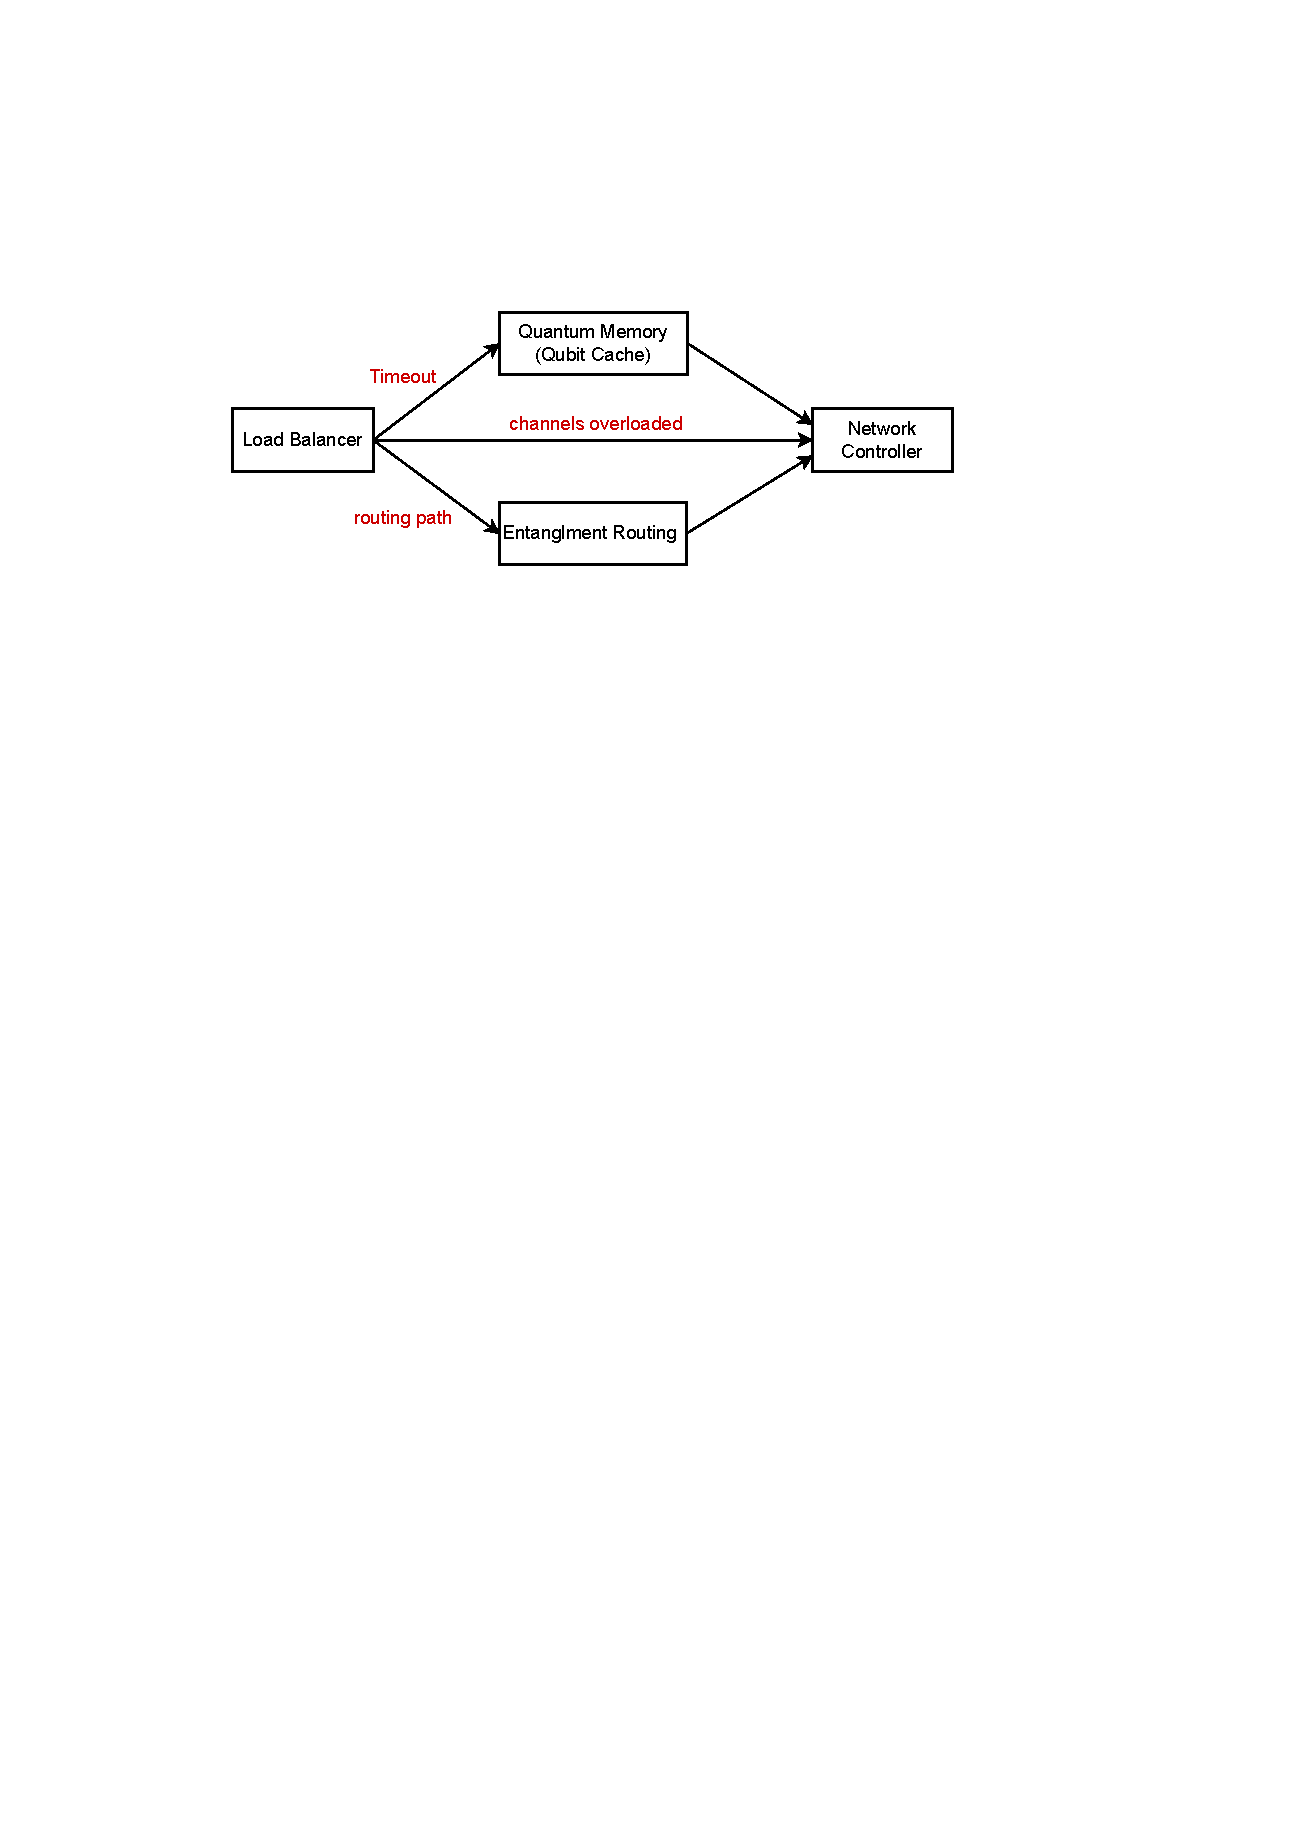
\includegraphics[width=1\linewidth]{images/pip.pdf}
     \caption{Example of a QNFV pipelet}
     \label{fig:future}
\end{figure}

\subsubsection{Q2 Interface} The global SDN controller specifies how traffic should be processed using pipelets. Each of these pipelets would define a quantum traffic class and a corresponding directed acyclic graph (DAG) that would represent the processing sequence by QNFs. The quantum traffic class subset of the input traffic would be specified by the pipelets. The DAG would be composed of nodes (QNFs or external ports) and edges (type of traffic).

\subsubsection{Q2 Internal Operation} The pipelets would dictate traffic processing but not the physical implementation in the specific quantum computing cluster. We propose there to be three internal components for Q2: (i) the scaling component which would compute and dynamically adapt the number of QNF instances based on traffic demand; (ii) the placement component which would Assign QNF instances to specific quantum computing servers; and (iii) the interconnection component which would configure the quantum network to route traffic across the appropriate QNF instances. 

\subsection{\textit{Q2 System Architecture}}

\begin{figure}[H]
     \centering
     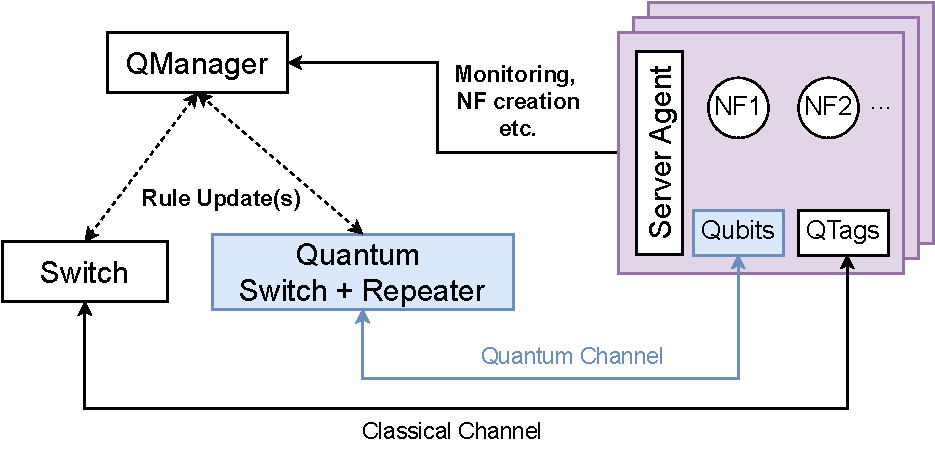
\includegraphics[width=0.9\linewidth]{images/E2toQuantum.pdf}
     \caption{Proposed Q2 Architecture}
     \label{fig:future}
\end{figure}

\subsubsection{Q2 System API}  
We propose a declarative policy formulation where operators would be able to express policies via pipelets, describing how a particular quantum traffic class should be processed. The pipelet structure would contain a quantum traffic class. The traffic class would be defined using the header fields and physical ports of classical tag of the quantum packet. The Directed Acyclic Graph (DAG) would represent the processing sequence of the traffic through QNFs. The nodes of the DAG would represent QNFs or physical ports and the edges would describe quantum traffic flow between nodes.

\subsubsection{Q2 System Inputs}
We propose that Q2 would require 2 main inputs in addition to the pipelets.  The first input would be the description of the QNFs which would be provided by the developers. The second input would be the description of the quantum network and compute hardware. These two inputs are proposed as they are the vital for Q2 to determine for efficient scheduling and routing quantum packets through the QNFs.

\subsubsection{Q2 System Components}
We propose the Q2 system to have three major components:
\begin{itemize}
    \item Q2 Manager: Will oversee the overall operation of the quantum cluster and interface with quantum switches and Q2 Server Agents.
    \item Q2 Server Agent: will manage operations within each quantum server.
    \item Q2 Dataplane (Q2D): will act as a software traffic processing layer underlying the QNFs at each server.
\end{itemize}

\subsection{\textit{Q2 Dataplane (Q2D)}}
We propose the Q2 Dataplane, to be built on quantum switches, which would provide a flexible and high-performance data plane tailored for QNFV requirements. By leveraging a SDN based quantum switch \cite{quantumswitch_sdn} and extending its capabilities with custom modules and APIs, Q2D will aim to optimize quantum network function processing and attempt to ensure efficient resource utilization and dynamic scalability within the Q2 framework.

\subsection{\textit{Q2 Control Plane}}
We theorize the Q2 control plane to manage several critical functions within the system, including the placement of Quantum Network Functions (QNFs), their interconnection, dynamic scaling based on load, and ensuring QNF affinity constraints.

\subsubsection{QNF Placement}
The initial placement of QNFs is proposed to involve the following series of steps:
\begin{enumerate}
    \item \textbf{Merging Pipelets into a Single Policy Graph:} Q2 will combine all input pipelets into a single policy graph, or pGraph, which would be the union of individual pipelets. Each node in this graph would represent a QNF, and edges represent would traffic flows between them.
    \item \textbf{Sizing Load and Capacity Estimates:} Q2 shall use initial load estimates (incoming traffic streams) and per-core capacities from QNF descriptions to determine the number of QNF instances needed. The estimates will be used as a starting point for system bootstrapping, with adjustments made dynamically based on actual load.
    \item \textbf{Converting the pGraph to an iGraph (Instance Graph):} The pGraph will be transformed into an instance graph (iGraph), where each node represents an instance of an QNF. This involves splitting nodes and distributing input traffic across instances while respecting affinity constraints. Additionally, when splitting multiple adjacent nodes, affinity constraints can lead to optimizations by minimizing the number of edges between QNF instances, enhancing placement efficiency.
    \item \textbf{Instance Placement:} The goal is to minimize inter-server traffic, as intra-server forwarding incurs lower delay and consumes fewer resources.
    Q2  will treat instance placement as a graph partition problem, using a modified Kernighan-Lin heuristic for optimization. The process will involve: starting with a valid solution obtained by bin-packing vertices into partitions based on a depth-first search. Then, iteratively swapping pairs of vertices from different partitions to reduce cross-partition traffic until no further improvement is possible. 
    For new NF instances, the algorithm is simpler due to migration avoidance. It would involve placing new instances in the partition that incurs the least cross-partition traffic.
\end{enumerate}

\subsubsection{Service Interconnection}
In the Q2 system, service interconnection is hoped to ensure proper traffic steering between QNF instances based on predefined filters annotated in the policy graph (pGraph) and instance graph (iGraph). This process would involve three main stages:
\begin{enumerate}
    \item \textbf{Instantiating QNF Ports:} Specifies the number of output ports and the traffic attributes associated with each port. The role of Q2D here would be to instantiate virtual ports (vports) according to the QNF description and the iGraph.
    
    \item \textbf{Adding Quantum Traffic Filters: } If an edge requires only a subset of the traffic generated by the QNF instance, Q2 will insert an additional classification stage in the Q2D. This would ensure that only traffic matching the edge filters is forwarded.

    \item \textbf{Configuring the Quantum Switch and Q2D:} Q2 will configure the switch and Q2D to attach QNF ports to edges and instantiate the necessary filters. Local edges within one server would be handled by Q2D alone, while inter-server edges route through Q2D to physical quantum routers.
\end{enumerate}

\subsubsection{Dynamic Scaling - Load Balancing}
Dynamic scaling shall address changing loads and the need to split the load across multiple QNF instances when a single instance becomes insufficient. Q2 will have the ability to detect an overload based on queues and processing delays, and also QNFs shall report their instantaneous load. Upon overload, the Server Agent shall notifiy the Q2 Manager, which will use an incremental algorithm to place new QNF instances. This would involve setting up new interconnection states and consider flow affinity requirements.Finally, incoming traffic would be correctly split across new and existing instances, ensuring continuity and efficiency.

\section{Prototype Implementation}

\begin{figure*}
     \centering
     \begin{subfigure}[b]{0.475\textwidth}
         \centering
         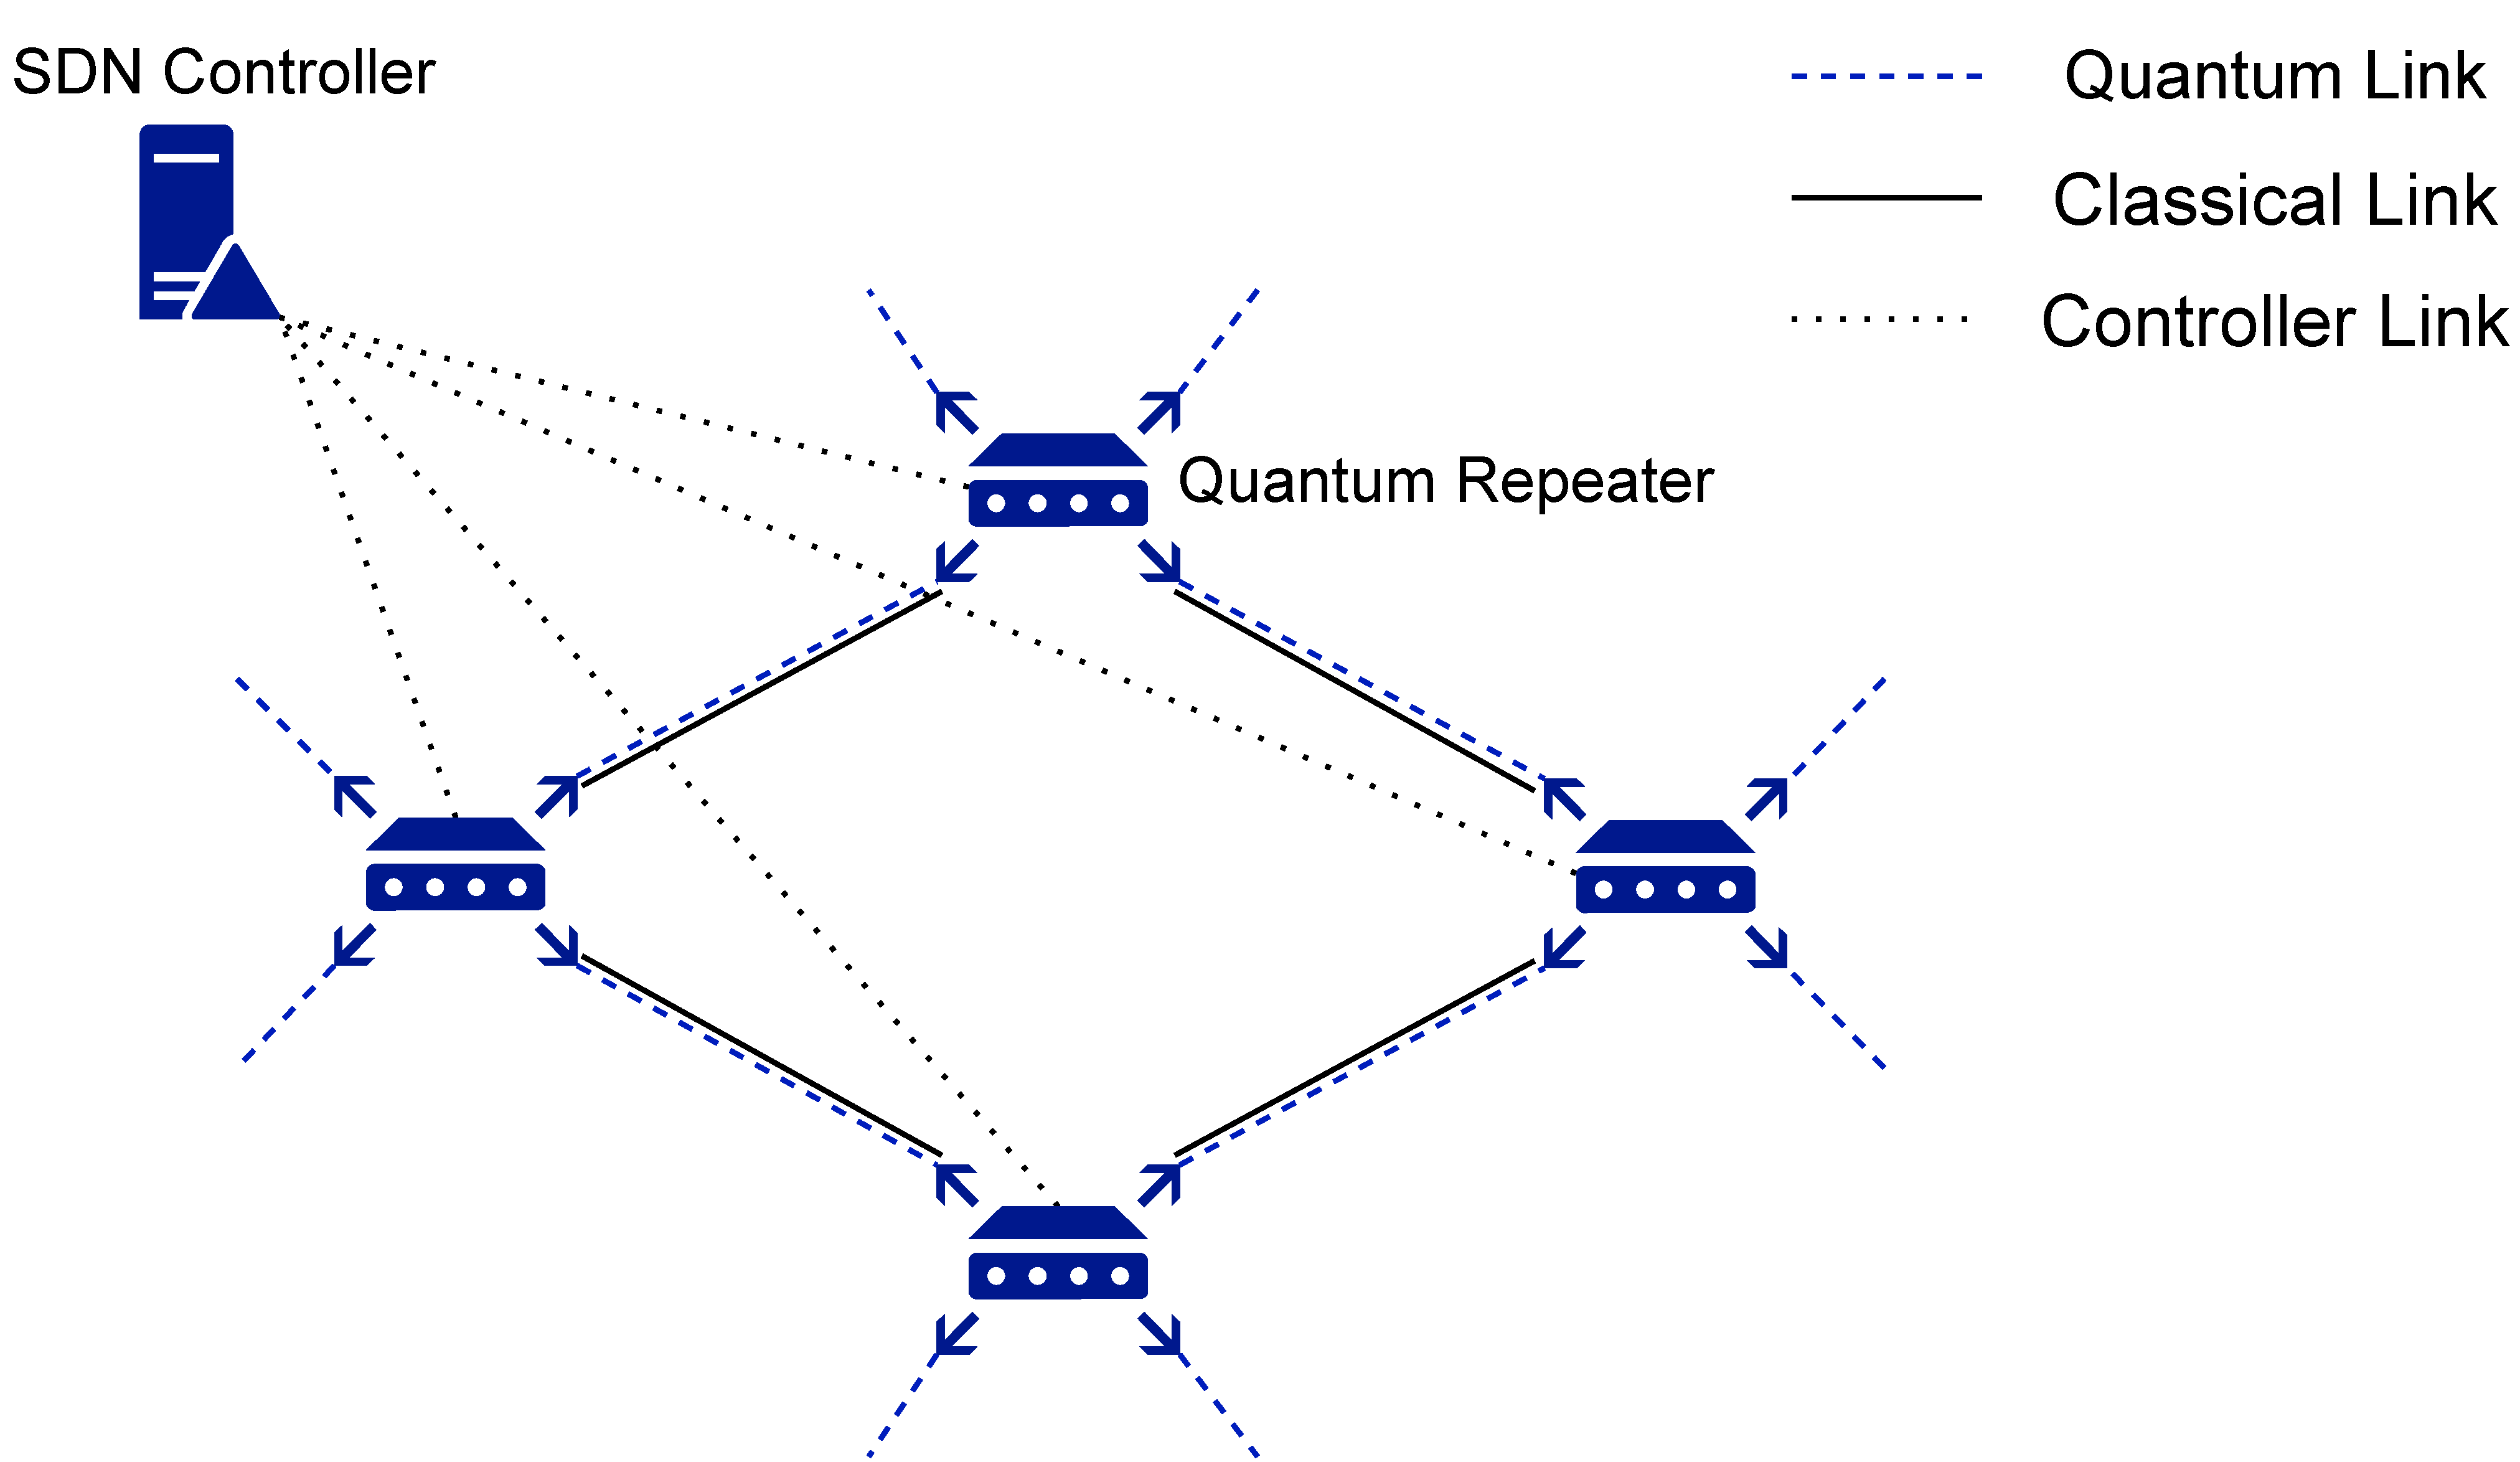
\includegraphics[width=0.9\linewidth]{images/net.pdf}
         \caption{Overview of theoretical quantum network}
         \label{fig:net}
     \end{subfigure}
     \begin{subfigure}[b]{0.475\textwidth}
         \centering
         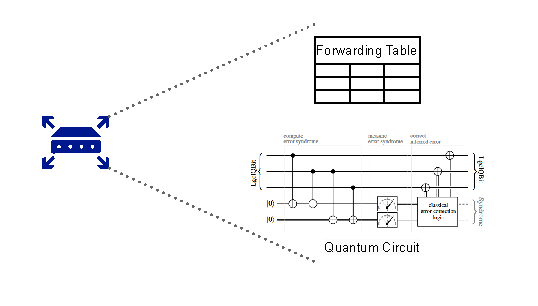
\includegraphics[width=0.9\linewidth]{images/QR.pdf}
         \caption{Proposed implementation of Quantum Repeater}
         \label{fig:router}
     \end{subfigure}
\end{figure*}


\subsection{Quantum Network Simulation}
To build the backbone of our proof-of-concept virtualization of quantum network functions, we employed NetSquid \cite{Coopmans_2021} and QuNetSim \cite{Diadamo_2021}, a widely-used quantum network simulator. NetSquid \& QuNetSim offer a comprehensive suite of tools for simulating quantum networks, enabling us to model and analyze the behavior of quantum components and their interactions accurately. By leveraging NetSquid \& QuNetSim, we simulated the operations of quantum repeaters, entanglement distribution, and quantum error correction mechanisms within a controlled environment. This provided a robust platform to validate the design and capabilities of our framework to support various quantum network functions.

\subsection{Modified Quantum Repeater}
In our implementation, we made modifications to the standard quantum repeater simulation within NetSquid. We enhanced the repeaters to support programmable forwarding tables that dictate the routing of qubits based on predefined policies. Additionally, we integrated quantum circuits capable of performing essential network functions such as entanglement swapping, quantum error correction, and state purification. These modifications transformed the repeaters from simple relay devices into sophisticated nodes capable of executing complex quantum network functions, thereby enabling the virtualization of these functions across the network.

\subsection{Implementing QNFVs}
We developed a Software Defined Network (SDN) controller (Q2 Manager) to manage and orchestrate the virtualized network functions over the quantum network. This controller provides a centralized management interface, offering a global view of the network and enabling dynamic control over its operation. The SDN controller communicates with the quantum repeaters, sending instructions for routing qubits and configuring quantum circuits as needed. By abstracting the control plane from the underlying hardware, the SDN controller facilitates flexible and efficient network management, akin to classical SDNs but adapted for the unique challenges of quantum networks. This approach allows us to dynamically allocate resources, optimize network performance, and ensure reliable quantum communication.

\section{Evaluation}

\subsection{Benchmarking Challenges}
Given the nascent stage of quantum cloud network architectures, we cannot currently benchmark our setup against existing architectures. The lack of established frameworks and standardized metrics for quantum networks means that we cannot apply traditional benchmarking approaches directly. Instead, to demonstrate the feasibility and effectiveness of our proposed framework, we conducted a sample test. This test aims to showcase the fundamental capabilities of our implementation in a controlled scenario, providing an initial validation of our design.
\subsection{Quantum Entanglement Distribution and Error Correction Test}
For our sample test, we ran a quantum entanglement distribution experiment combined with a simple error correction code. This test involved generating entangled qubit pairs and distributing them across the simulated quantum network using our modified repeaters and SDN-controlled routing. During the distribution process, we employed basic error correction techniques to mitigate the effects of noise and decoherence, ensuring the integrity of the entangled states. The successful completion of this test demonstrated the practical viability of our framework in managing quantum network functions. It highlighted the framework's ability to support essential operations such as entanglement distribution and error correction, thereby validating our approach to virtualizing quantum network functions. The results of this test provide a strong foundation for further development and optimization of our framework, paving the way for more complex and scalable quantum cloud networks.

\section{Future Work}
Future research will focus on enhancing the scalability and robustness of our framework. We aim to develop more sophisticated error correction techniques, optimize resource allocation, and explore the integration of advanced quantum algorithms. Additionally, we plan to conduct extensive simulations and real-world experiments to further validate and refine our approach, ultimately paving the way for the practical deployment of quantum cloud networks.

\section{Conclusion}
This paper presents a framework for a quantum cloud network, leveraging current quantum computing network components to anticipate the architecture and requirements of future quantum clouds. Using NetSquid for simulation, we modified quantum repeaters to handle forwarding and quantum circuit operations. Additionally, we developed an SDN controller to manage the network, enabling virtualized quantum network functions. Although benchmarking against existing architectures is not yet possible, our sample test of quantum entanglement distribution with error correction demonstrates the feasibility and potential of our framework.



\bibliographystyle{plain}
\bibliography{IOPEXPORT_BIB}

\end{document}

